%*******************************************************************************
%*********************************** Chapter DUNE ******************************
%*******************************************************************************
\chapter{The Deep Underground Neutrino Experiment}  %Title of chapter

\graphicspath{{DUNE/Figs/PDF/}{DUNE/Figs/Raster/}{DUNE/Figs/Vector}}

\nomenclature[a-tick]{tick}{Unit of time equal to 500 ns}
\nomenclature[z-CRC]{CRC}{Cosmic Ray Counter}
\nomenclature[z-SiPM]{ADC}{Analogue to Digital Converter}
\nomenclature[z-TPC]{TPC}{Time Projection Chamber}
\nomenclature[z-SiPM]{SiPM}{Silicon Photo Multiplier}
\nomenclature[z-FD]{FD}{Far Detector}

%********************************** %First Section  **************************************
\section{DUNE location and beam line} %Section - X.1 

%********************************** %Second Section  *************************************
\section{The DUNE detectors and schedule} \label{sec:DUNEDetector} %Section - X.2

%********************************** %Third Section  *************************************
\section{Physics opportunities of DUNE} %Section - X.3

%********************************** % 3.1 Section  *************************************
\subsection{Neutrino physics}  %Section - X.3.1

%********************************** % 3.2 Section  *************************************
\subsection{Nucleon decay and supernovae neutrinos}  \label{sec:NDK_Atmos}%Section - X.3.2

\begin{table}[h!]
\caption[Nucleon decay limits in DUNE and Super-Kamiokande]
        {Nucleon decay limits in DUNE and Super-Kamiokande, in some favoured decay channels.}
\centering
\label{tab:NDKLim}
\begin{tabular}{c c c c}
\toprule
{Total flux (cm$^{-2}$ s$^{-1}$)} & {Mean E$_{\mu}$ (GeV)} & {Mean slant depth (m w.e)} & {Mean $\theta$ ($^{\circ}$)} \\ 
\midrule
5.66 $\times$ 10$^{-9}$           & 283                    & 4532                       & 26                           \\
\bottomrule
\end{tabular}
\end{table}

%********************************** % 3.3 Section  *************************************
\subsection{Background to nucleon decay} \label{sec:BkNDK}  %Section - X.3.3

\begin{figure}[h]
  \centering
  %\includegraphics[width=0.85\textwidth]{}
  \caption[How the interaction of a cosmic muon can mimic a nucleon decay signature]
          {How the interaction of a cosmic muon can mimic a nucleon decay signature, by producing a $K^{0}_{L}$ which interacts far from the detector wall, producing an isolated kaon.}
  \label{fig:35tonWireGeom}
\end{figure}

%********************************** % Fourth Section  *************************************
\section{Path to building DUNE - The 35 ton prototype} \label{sec:The35tonDetector}  %Section - X.4

\begin{figure}[h]
  \centering
  %\includegraphics[width=0.85\textwidth]{}
  \caption[The wrapped wires of the 35 ton]{A schematic showing what the wrapped wire planes of the DUNE detector designs looked like in the 35 ton.}
  \label{fig:35tonWireGeom}
\end{figure}

\begin{figure}[h]
  \centering
  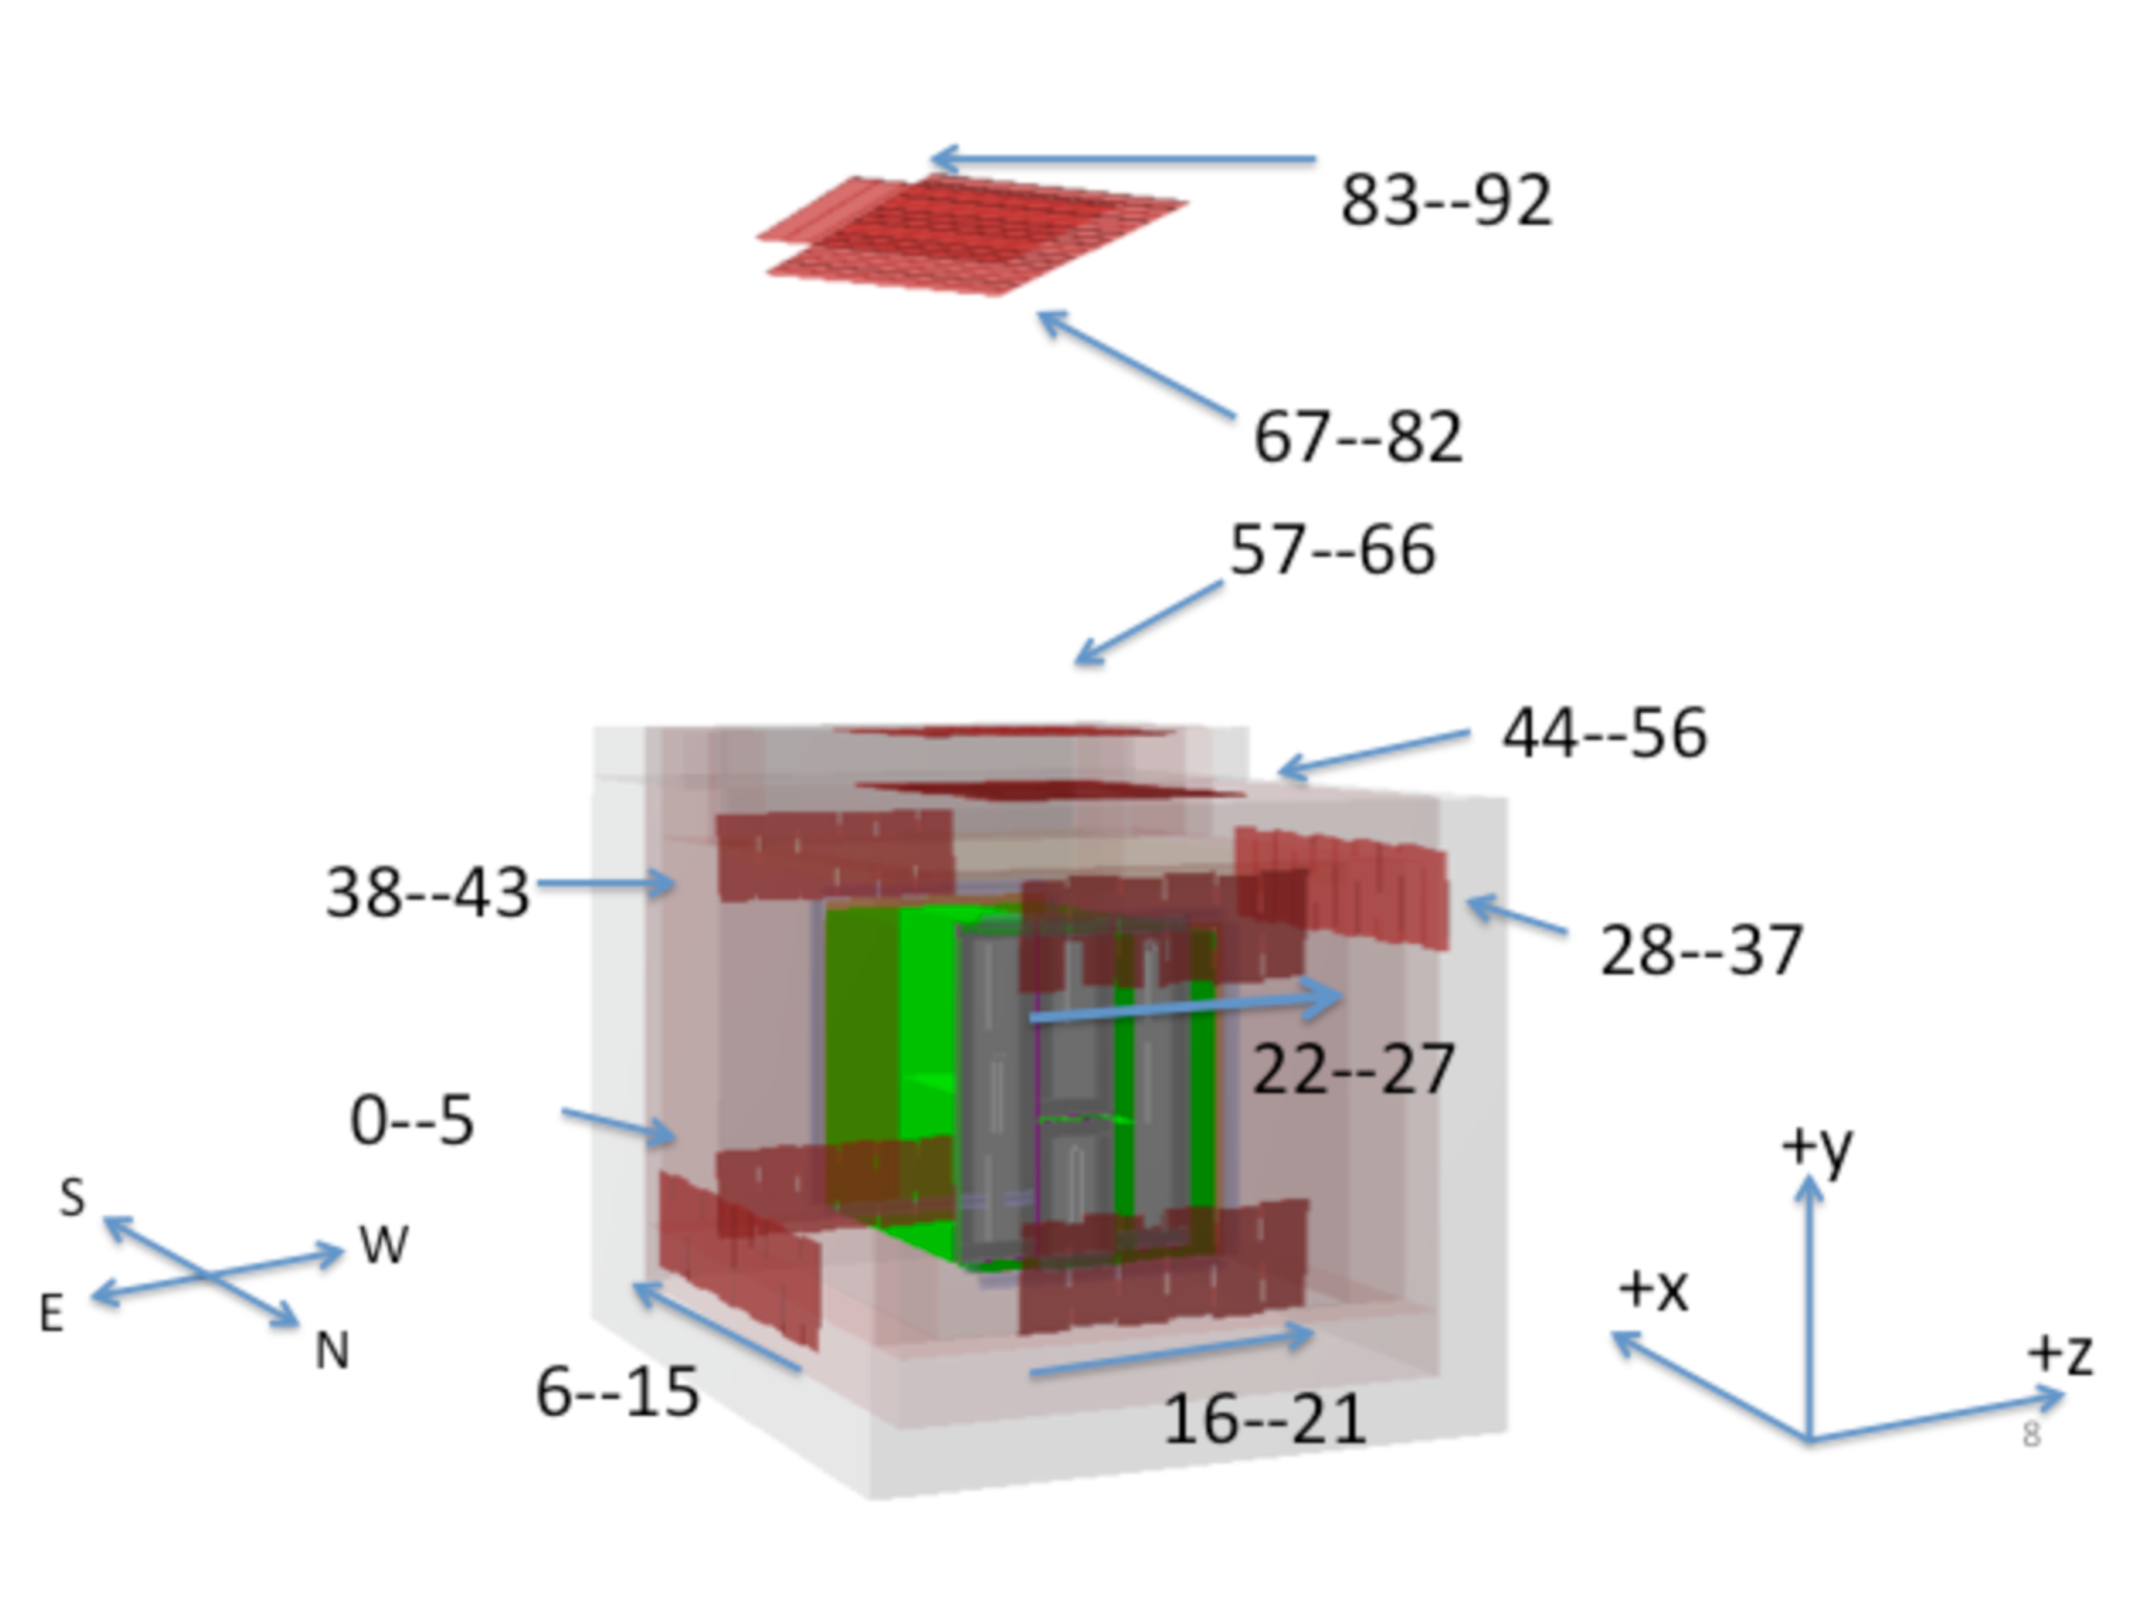
\includegraphics[width=0.85\textwidth]{35tonFullDetect}
  \caption[A representation of the counter locations in the 35 ton]
          {A representation of the counter locations in the 35 ton, with the magnetic and LArSoft co-ordinate systems shown. The other detector components can be seen inside the cryostat, such that the counters on the North wall are behind the short drift volume. The East - West counters are numbered 6-15 and 28-37 respectively. The North Lower - South Upper counters are numbered 16-21 and 38 - 43 respectively. The North Upper - South Lower counters are numbered 22-27 and 0-5 respectively. The telescope triggers are numbered 44-92 and are split into four groups.}
  \label{fig:35tonCounterLoc}
\end{figure}

%********************************** % Fifth Section  *************************************
\section{The DUNE software} \label{sec:LArSoft} %Section - X.5
The software package used by DUNE is called LArSoft~\citep{Church_LArSoft}~\citep{LArSoftOrg} which is a simulation, reconstruction and analysis package for Liquid Argon Time Projection Chamber (LArTPC) that is being used by many experiments in the US neutrino program. LArSoft has been developed to be detector agnostic, meaning that much of the code is shared between experiments. To this end it is envisioned that it will be used as a platform for constant development in existing experiments and those still in the planning phases such as DUNE. LArSoft is built around the Fermilab-supported \emph{analysis reconstruction framework} (\emph{art}). External packages such as ROOT~\citep{ROOT} and GEANT4~\citep{GEANT4} are incorporated into LArSoft meaning that the user does not have to coordinate specific versions of the packages as the newest versions are automatically incorporated. \\

There are numerous mechanisms by which particles can be generated within the software with external packages. One such package is GENIE~\citep{GENIE} which is used to study neutrino interactions and nucleon decays. Another package, Nuance~\citep{Nuance}, is a neutrino interaction generator specifically for Liquid Argon (LAr). Finally, CRY~\citep{CRY} and CORSIKA!!!citep{CORSIKA} are cosmic ray events generators which are used to simulate the expected event rates for surface detector locations in absence of a neutrino beam. Recently the MUon Simulations UNderground (MUSUN)~\citep{MUSUN}~\citep{MUSUN2} generator which takes the output of MUon SImulation Code (MUSIC)~\citep{MUSUN}~\citep{MUSIC}~\citep{MUSIC2} has also been incorporated, see Section~\ref{sec:FDIncorporation} for further details. It is also possible to use an inbuilt single particle generation mode which is fully tunable as particle type, momenta, positions and directions can all be varied. \\

The co-ordinates and angles in LArSoft are defined as follows, and schematic representations of how this appears in the 35 ton are shown in Figure~\ref{fig:LArSoft_coords}:
\begin{itemize}
\item $x$ - The beam direction, with maximal $x$ being where the beam enters the detector.
  \begin{itemize}
  \item In the 35 ton prototype where there is no beam positive $x$ is in the opposite direction to that which electrons drift in the large TPC, where $x$ = 0 is the position of the APA frames in the long drift volume.
  \item In the far detector geometry $x$ = 0 is defined as the midpoint between the two rows of CPAs 
  \end{itemize}
\item $y$ - The vertical direction, with maximal $y$ being the most highest point.
  \begin{itemize}
  \item In the 35 ton $y$ = 0 is halfway between the gap created by the two centre APAs which are mounted one above the other.
  \item In the far detector $y$ = 0 is defined as the midpoint between the two vertical layers of TPCs.
  \end {itemize}
\item $z$ - Defined as such to have a right handed co-ordinate system.
  \begin{itemize}
  \item In the 35 ton $z$ = 0 is at the edge of the leftmost APA frame when looking down the long drift volume.
  \item In the far detector $z$ = 0 is defined at the edge of the leftmost APA frame when looking down the long drift volume.
  \end{itemize}
\item $\theta$ - The angle that a vector makes from the $x$ axis in the $xy$ plane.
\item $\phi$ - The angle between the $z$ axis and the vector.
\end{itemize}

\begin{figure}[h]
  \centering
  \begin{subfigure}{0.45\textwidth}
    \centering
    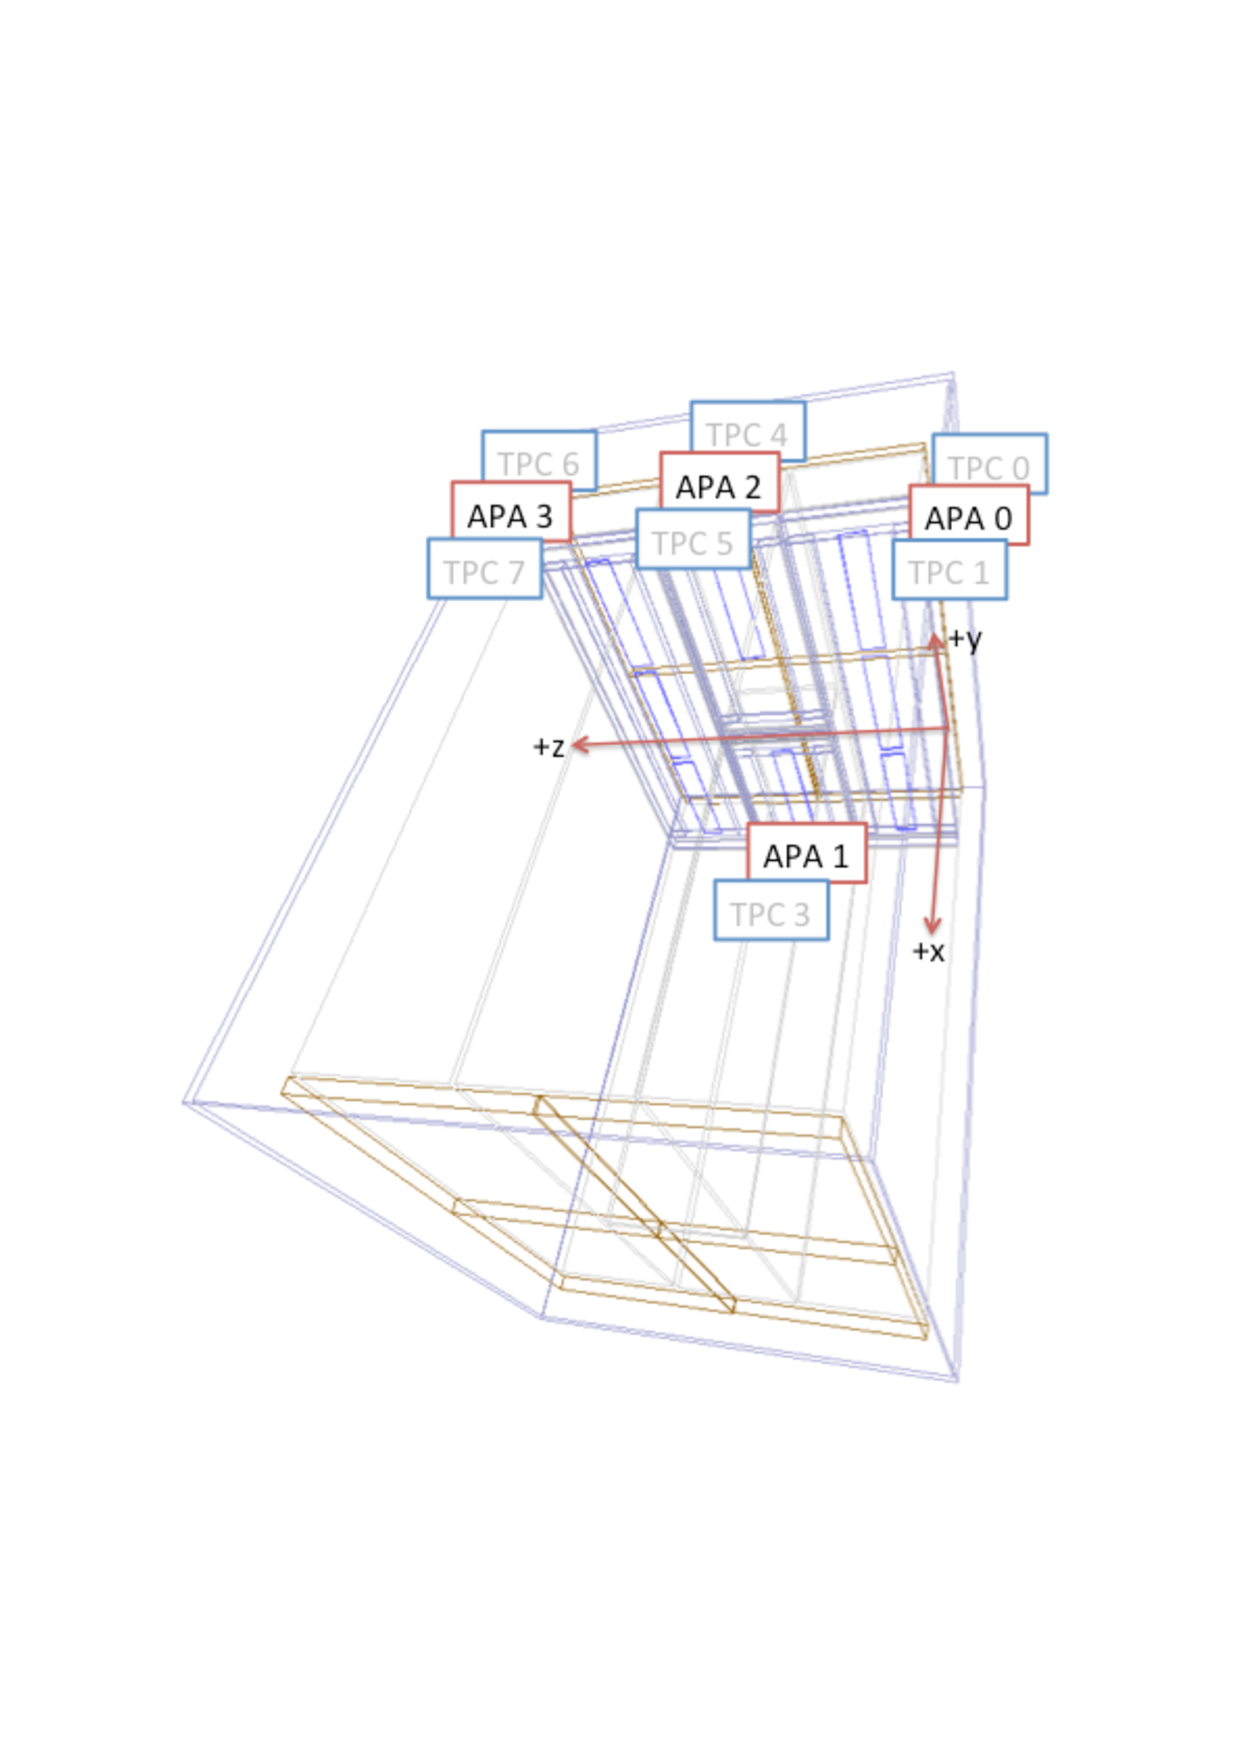
\includegraphics[width=\textwidth]{35ton_APASchem}
    \caption{The location of the origin of the 35 ton co-ordinate system in 3D.}
  \end{subfigure}
  \hspace{0.08\textwidth}
  \begin{subfigure}{0.45\textwidth}
    \centering
    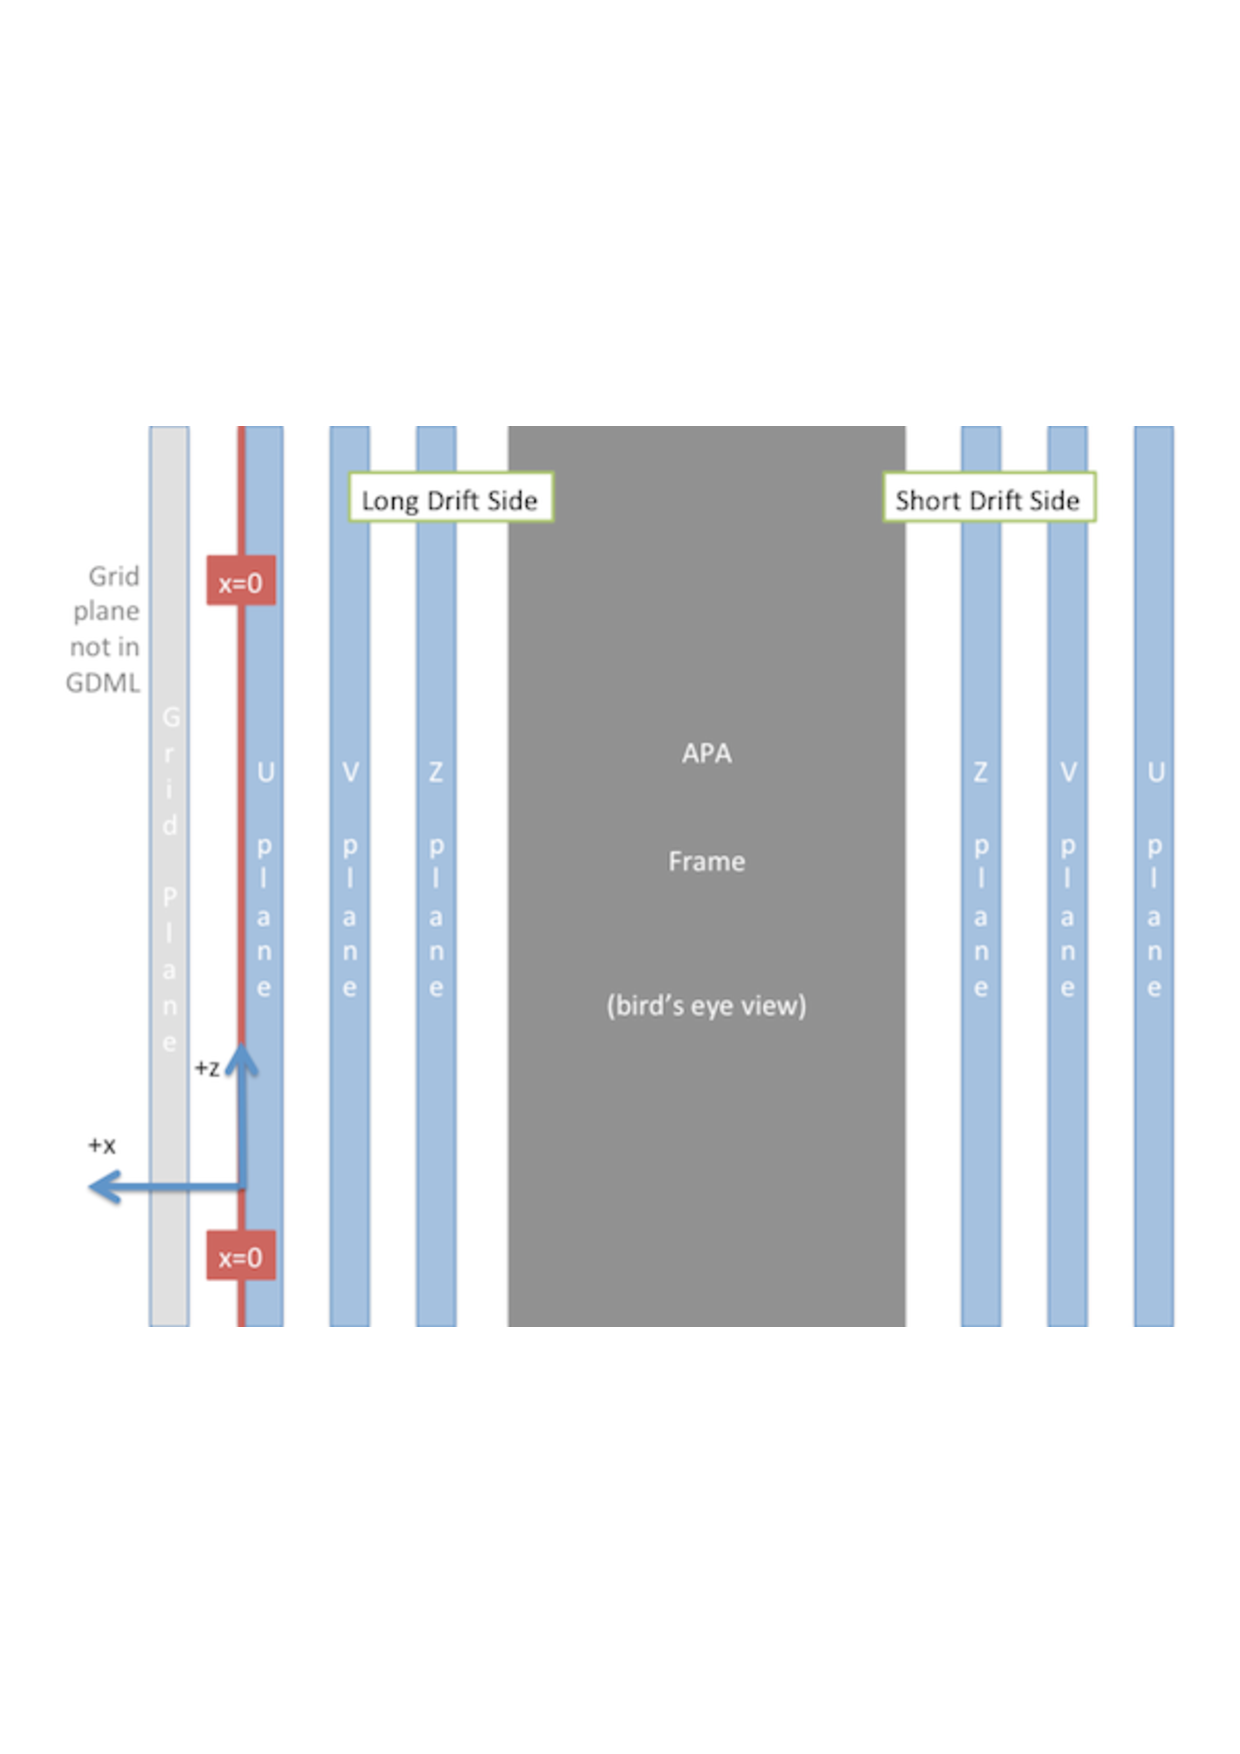
\includegraphics[width=\textwidth]{35ton_xCenter}
    \caption{The location of the origin of the 35 ton co-ordinate system in a 2D aerial view.}
  \end{subfigure}
  \caption[The LArSoft co-ordinate system as it is represented in the 35 ton.]
          {The LArSoft co-ordinate system as it is represented in the 35 ton. Left shows the location of the origin relative to the TPC detector components. The four APAs, and eight TPCs are shown, where the even numbered TPCs are on the short drift side, $\sim$20 cm drift, and the odd numbered TPCs are on the long drift side, $\sim$250 cm drift. The CPAs are also shown as the objects with a brown outline. Right shows the location of the origin with respect to the APAs. The wire planes are shown, the U and V planes are induction wires, whilst the Z planes are collection wires.}
  \label{fig:LArSoft_coords}
\end{figure}

The simulation of particles is usually split into five separate distinct processes to reflect the different stages in which development often progresses. The advantage of segmenting the computational process in this way is that improvements can easily applied to a file without rerunning the entire chain. This is especially important when large Monte Carlo or data samples are produced for general use within collaborations so that users are able to concentrate on improving a specific part of the computational process. When these all-purpose samples are produced the analysis performed provides users with any Monte Carlo truth information along with the reconstructed quantities for use in analyses performed outside LArSoft. The computational process is often broken down in the following way:
\begin{itemize}
\item Particle generator.
\item Particle transport using GEANT4.
\item Full detector simulation, including detector responses. 
\item Full event reconstruction.
\item Analysis.
\end{itemize}

Later significant focus will be given to the reconstruction of TPC data, and so it is necessary to briefly illustrate the mechanisms by which TPC data is reconstructed in LArSoft. Much of the information presented below is summarised in~\citep{LArSoftRecoNote}~\citep{LArSoftOrg}. After the full detector simulation or data taking, detector effects such as the electronics response function and a pedestal offset have to removed. Once these effects are removed the signal is estimated using the optimal value of $signal/noise$ which would produce the measured signal. This process, called deconvolution, does not conserve pulse height and is not guaranteed to preserve the normalisation. The deconvoluted signals are all unipolar distributions which means that Gaussian distributions can then be fitted to them when trying to reconstruct hits. This is shown in Figure~\ref{fig:LotsOfHits}, and explained further below.\\

\begin{figure}[h!]
  \centering
  \begin{subfigure}{0.95\textwidth}
    \centering
    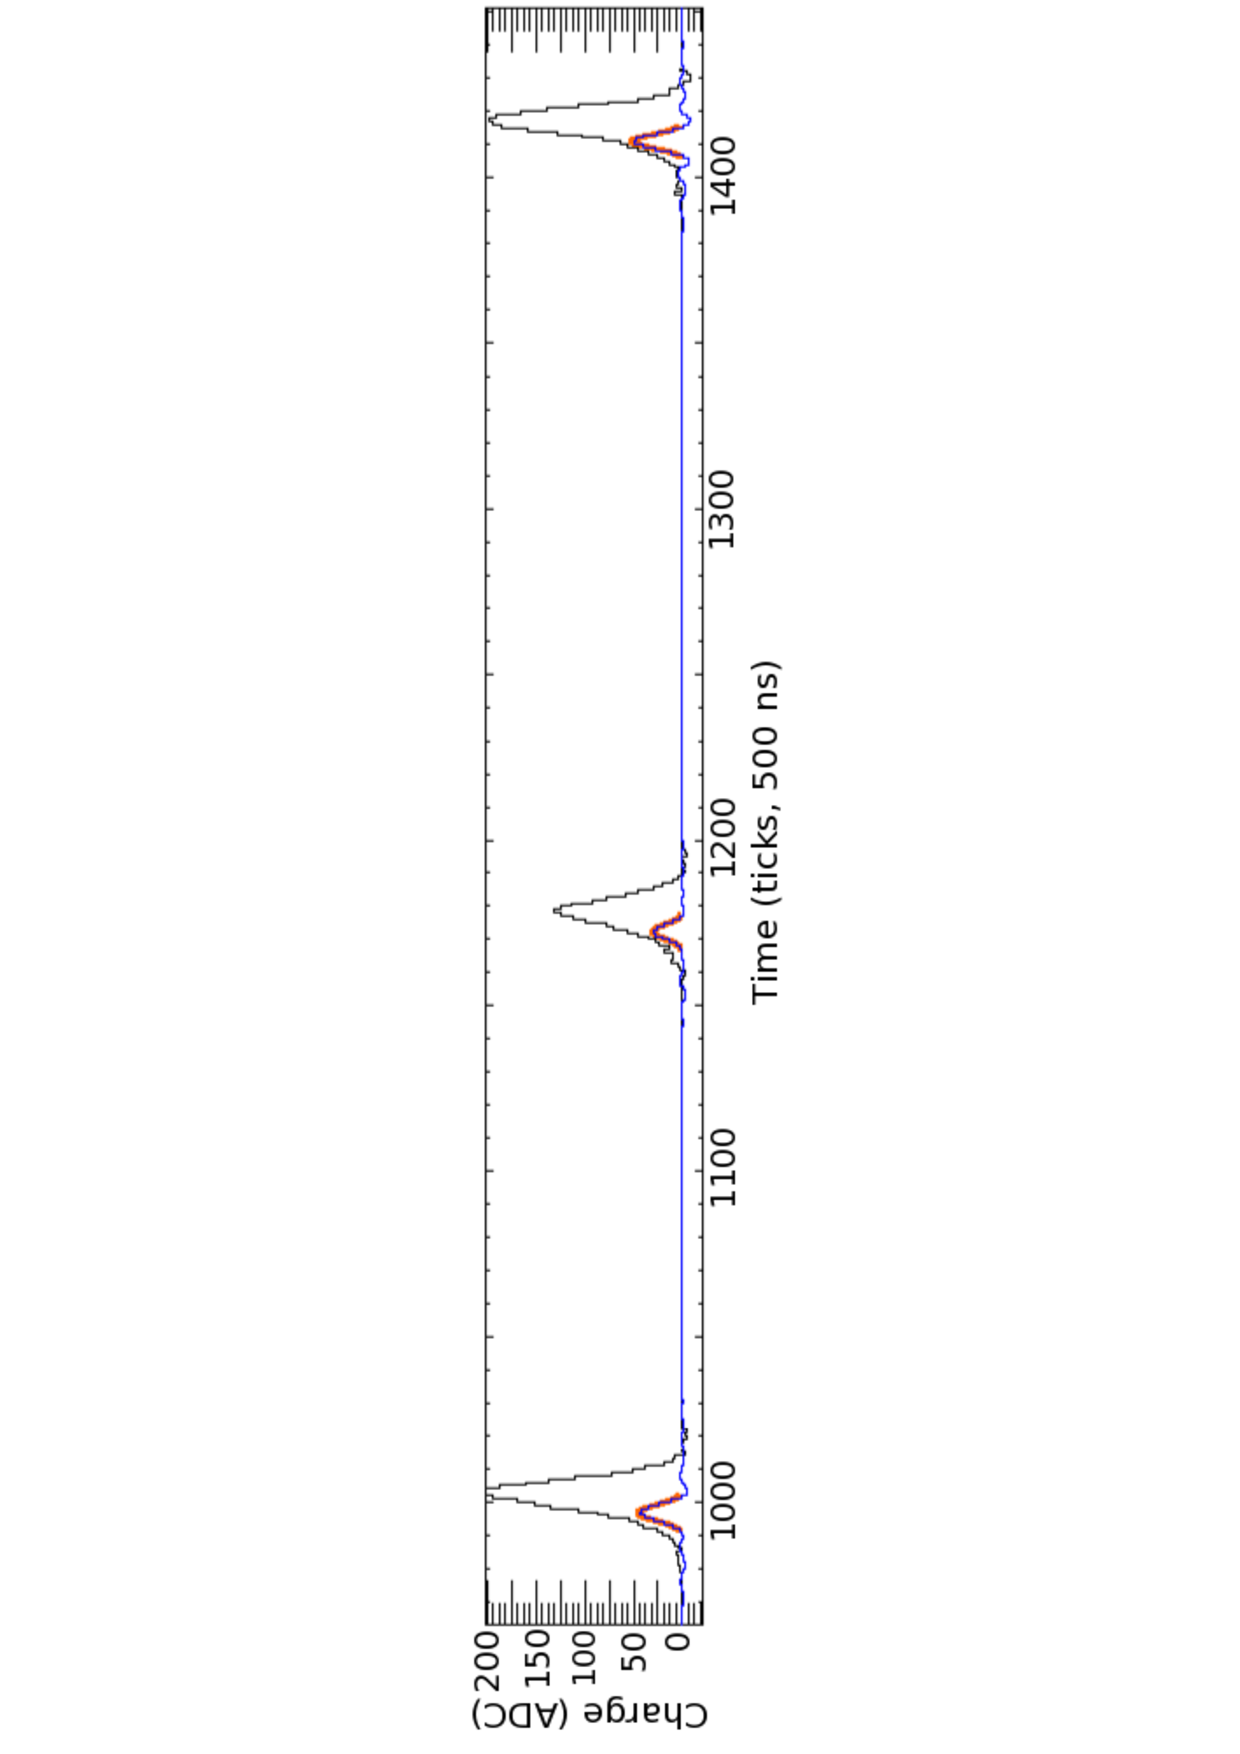
\includegraphics[width=\textwidth]{CollectionPlane}
    \caption{Collection plane depositions.}
    \label{fig:LotsOfHits_Col}
  \end{subfigure}
  \begin{subfigure}{0.95\textwidth}
    \centering
    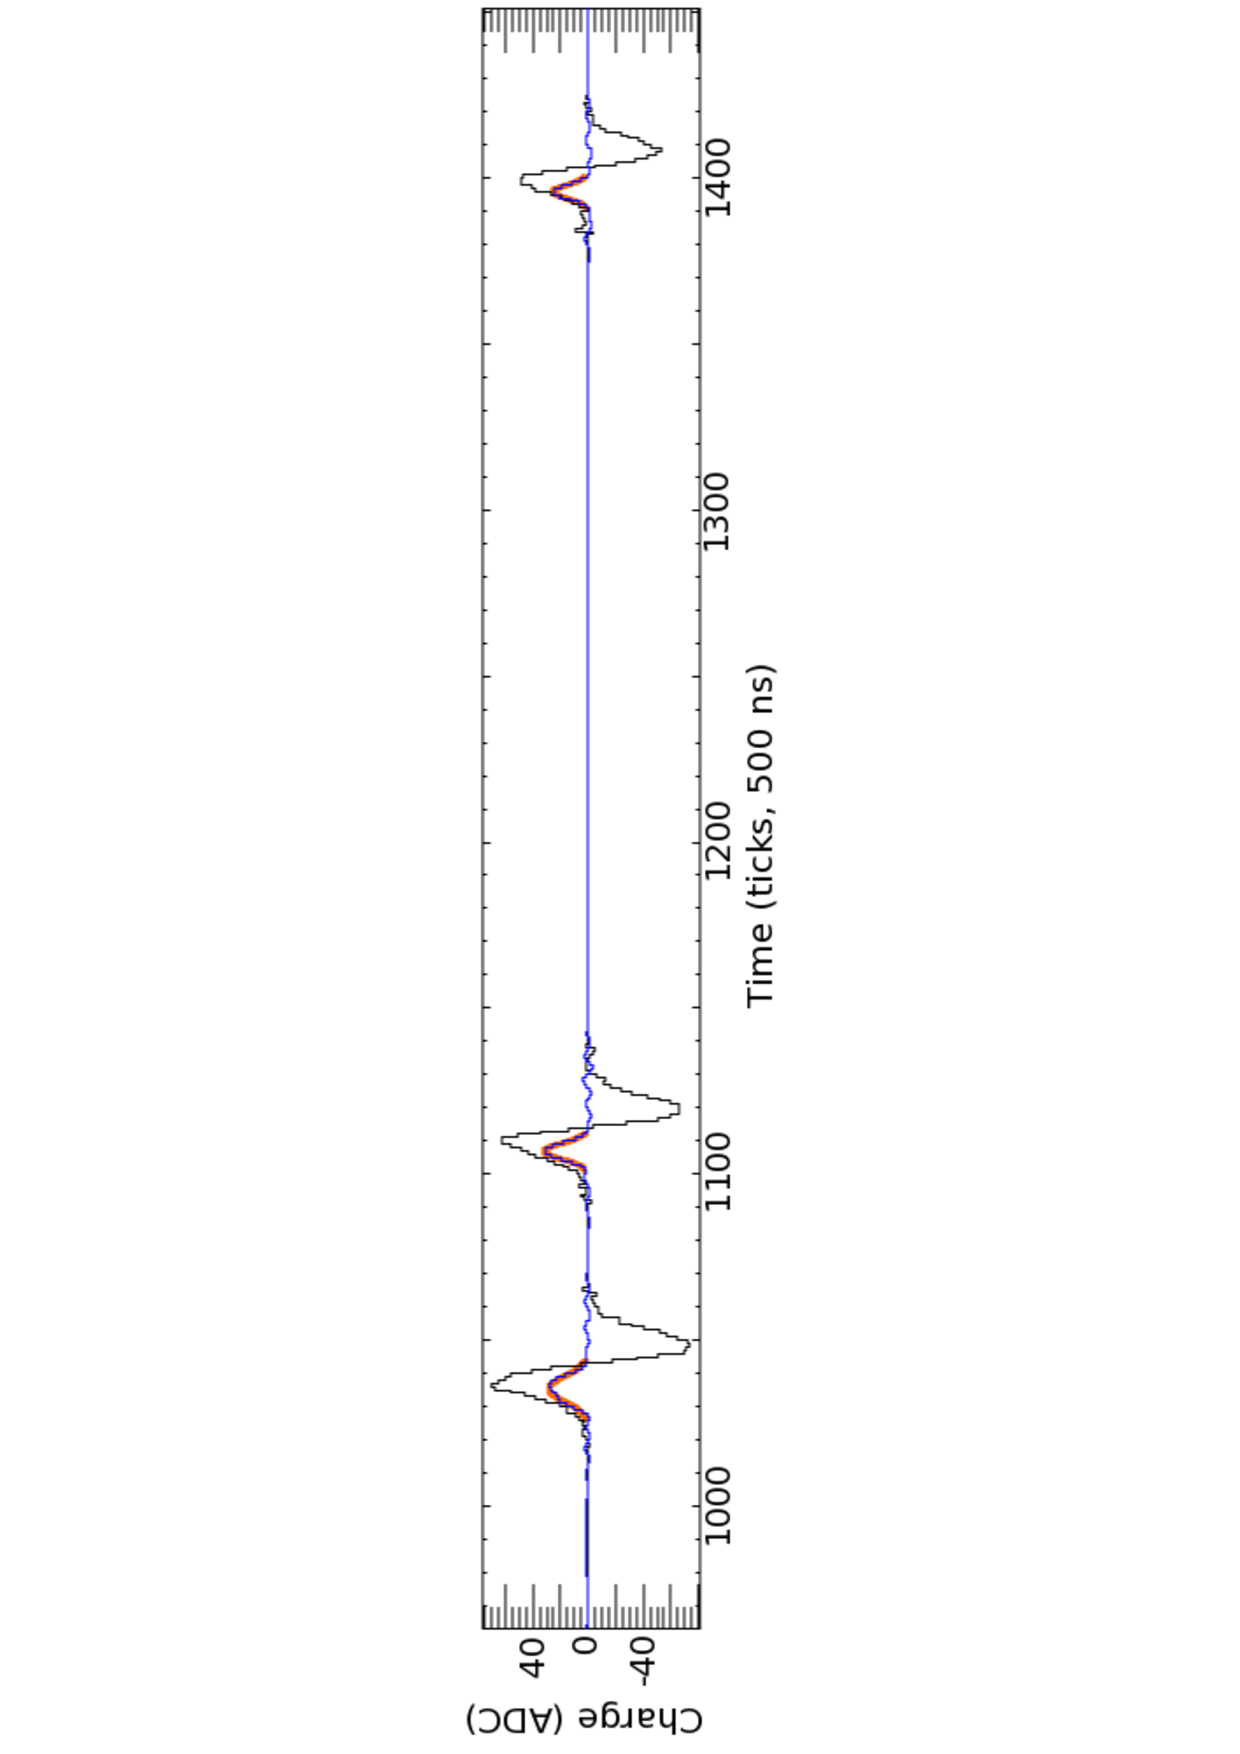
\includegraphics[width=\textwidth]{InductionPlane}
    \caption{Induction plane depositions.}
    \label{fig:LotsOfHits_Ind}
  \end{subfigure}
  \begin{subfigure}{0.95\textwidth}
    \centering
    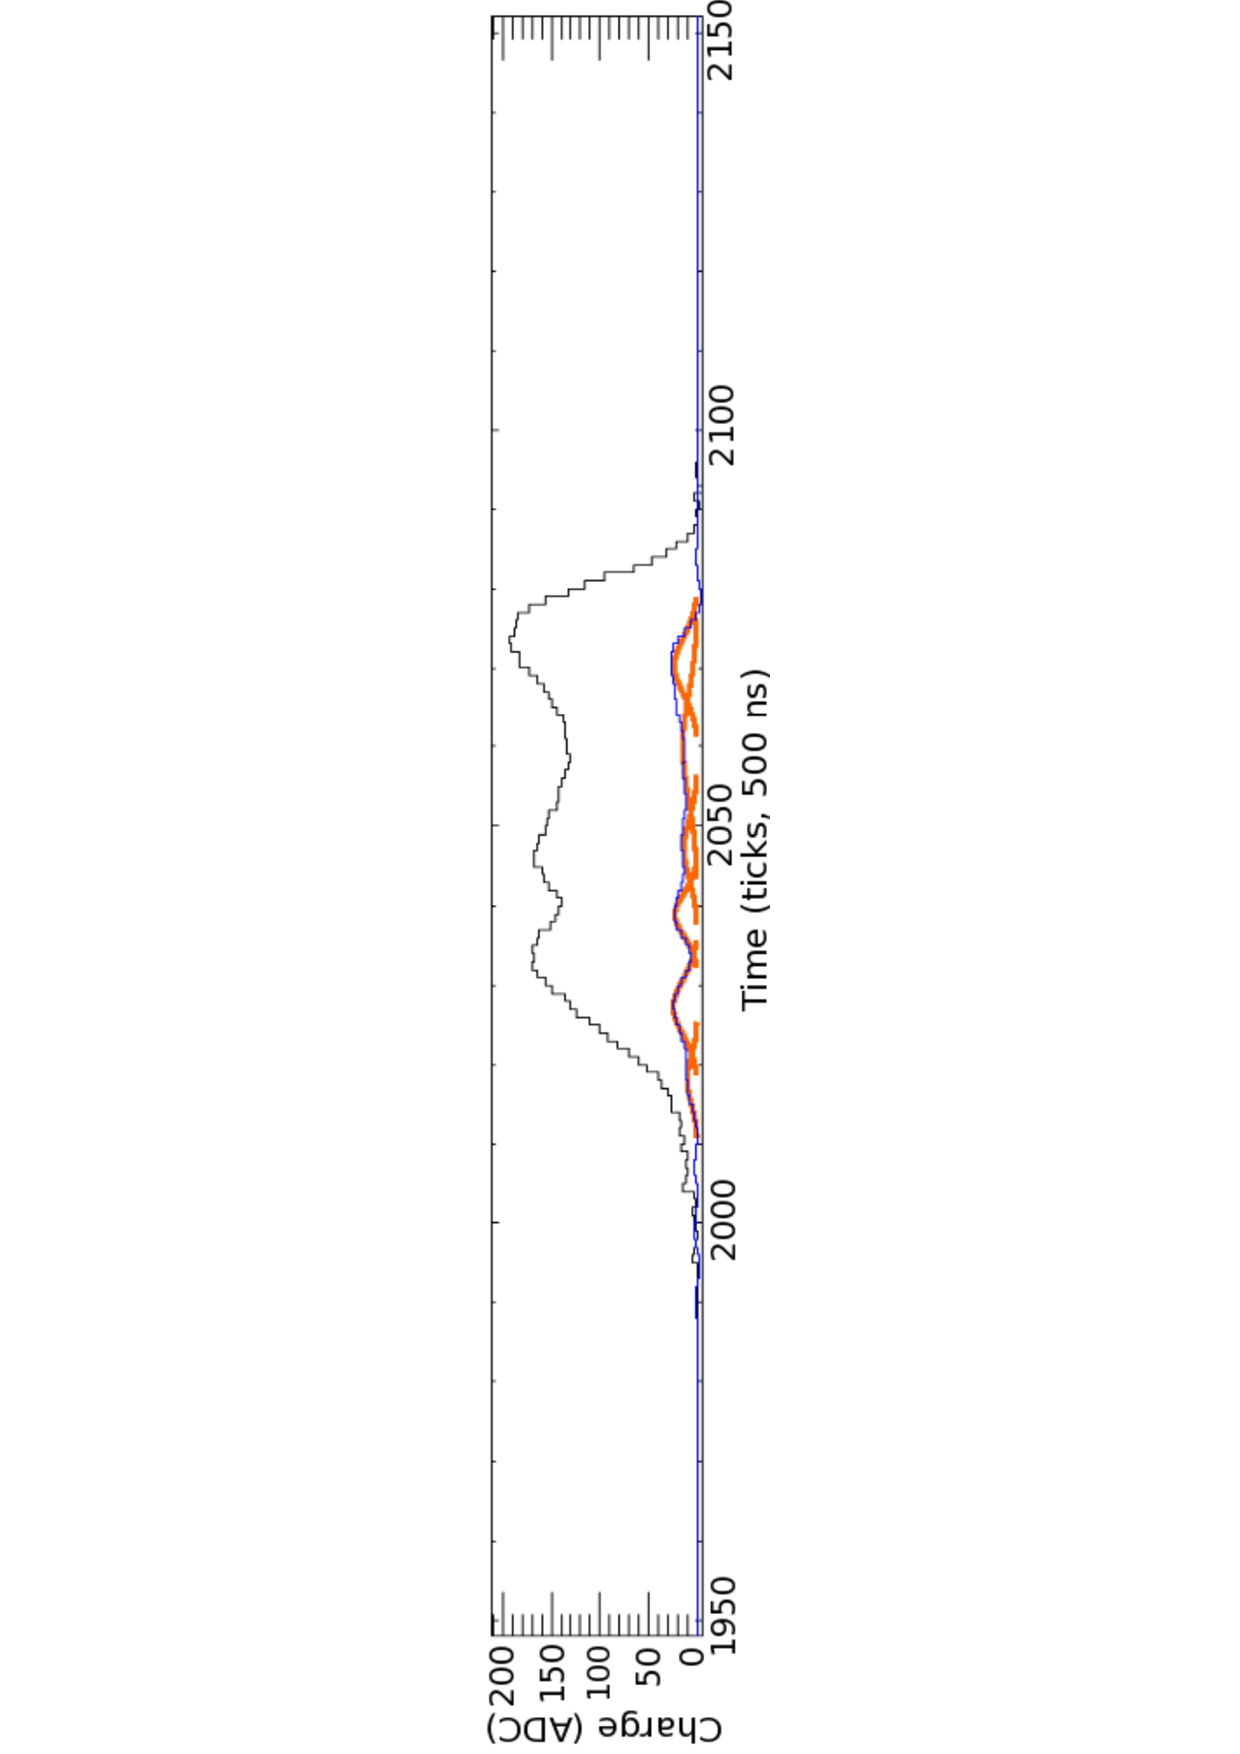
\includegraphics[width=\textwidth]{Complex}
    \caption{A large collection plane deposition over a large period of time.}
    \label{fig:LotsOfHits_Big}
  \end{subfigure}
  \caption[Reconstructed hits from simulated energy depositions]
          {The raw and deconvoluted signals with reconstructed hits on single wires for simulated energy depositions. The depositions, from particles generated by CRY, are not from a single event and have been selected for demonstration purposes only. The plots are shown with increasing charge (ADC) on the $y$ axis, and increasing time (ticks, 500 ns) on the $x$ axis. The black lines represent the raw signals, the blue lines represent the deconvoluted signals and the orange lines represent the reconstructed hits. Top shows depositions on a collection plane wire, it can be seen that the raw signal is unipolar. Middle shows depositions on an induction plane wire, it can be seen that the raw signal is bi-polar whilst the deconvoluted signal and reconstructed hits are unipolar. Bottom shows a complex deposition on a collection plane wire, where multiple reconstructed hits are required to reproduce the deconvoluted signal.}
  \label{fig:LotsOfHits}
\end{figure}

The deconvoluted signals are reconstructed into hits by identifying regions that are above a threshold value and then attempting to replicate the signal in these regions by introducing Gaussian distributions. For isolated hits this is typically achieved using only one Gaussian distribution, however for large energy depositions over a large period time where many particles are involved, multiple Gaussian distributions are often required. Large energy depositions are also possible when the direction of the particle aligns with a wire, this means that all of the deposited energy is collected on this single wire. Examples of reconstructed hits are shown in Figure~\ref{fig:LotsOfHits}. These figures are taken from separate CRY simulated events, and so do not correspond to a continuous simulated event. They have been selected only as a demonstration of the process of hit reconstruction. Figures~\ref{fig:LotsOfHits_Col} and~\ref{fig:LotsOfHits_Ind} show multiple time-separated energy depositions on a collection and induction wire respectively. A more complex energy deposition on a collection plane wire is shown in Figure~\ref{fig:LotsOfHits_Big} where energy depositions from many particles at similar times have created a complicated energy deposition that requires many reconstructed hits to explain. \\

As noted in Section~\ref{sec:DUNEDetector} and Section~\ref{sec:The35tonDetector} the DUNE FD and the 35 ton both have wrapped wires on the induction planes. A result of this is that the location of the reconstructed hit on an induction wire is ambiguous as a single wire has many wire segments, as shown in Figure~\ref{fig:35tonWireGeom}. An important feature of this ambiguity is that the TPC in which the hit occurred cannot be identified unless it is combined with another hit. These ambiguities do not extend to the collection plane wires as they are not wrapped and so consist of only a single wire segment in a single TPC. Hits are combined across the three planes by identifying wire segments on each plane which intersect and have hits at common times. In the traditional reconstruction process only hits that make these so-called 'triple points' are considered disambiguated, with other hits being identified as noise hits causing them to be discarded. \\

The inclination of the wire planes has to be carefully chosen so as to minimise both the number of wires required and the number of times that wire triplets intersect. This is shown in Figure~\ref{fig:WirePitches}, where the wire inclinations used in the 35 ton detector, are compared to those in the DUNE FD reference design. The inclination of wires in the 35 ton was 45$^{\circ}$ $\pm$ 0.7$^{\circ}$ meaning that many wire triplets cross twice and some wire pairs cross three times. When wire triplets cross multiple times the triplet which has the smallest distance between the common intersection point and the two, two-wire intersection points, is chosen as the best intersection candidate. This is shown as the 'Good intersection' on the right panel in Figure~\ref{fig:WirePitches}. The different wire pitches are necessary so that one of the triple points can be evaluated to be a better candidate, as with a wire pitch of 45$^{\circ}$ it can be impossible to distinguish between different triple points. The inclination of wires in the FD was chosen to be 36$^{\circ}$ to remove the possibility of multiple intersection points, as given the geometry of the APAs multiple intersection points are impossible and so disambiguation is much simpler. The lower inclination results in more induction wires being required though, making it more expensive to instrument the detector. It is also important that all wires on a given APA are either read at the top or base of the APA, depending on whether the APA is at either the top or the base of the detector respectively. This is because there must be minimal space between TPCs in the DUNE FD to reduce the internal dead space, and so TPCs cannot be read out along the sides as this would require a non-negligible amount of space to accomodate the cabling.\\

\begin{figure}[h!]
  \centering
  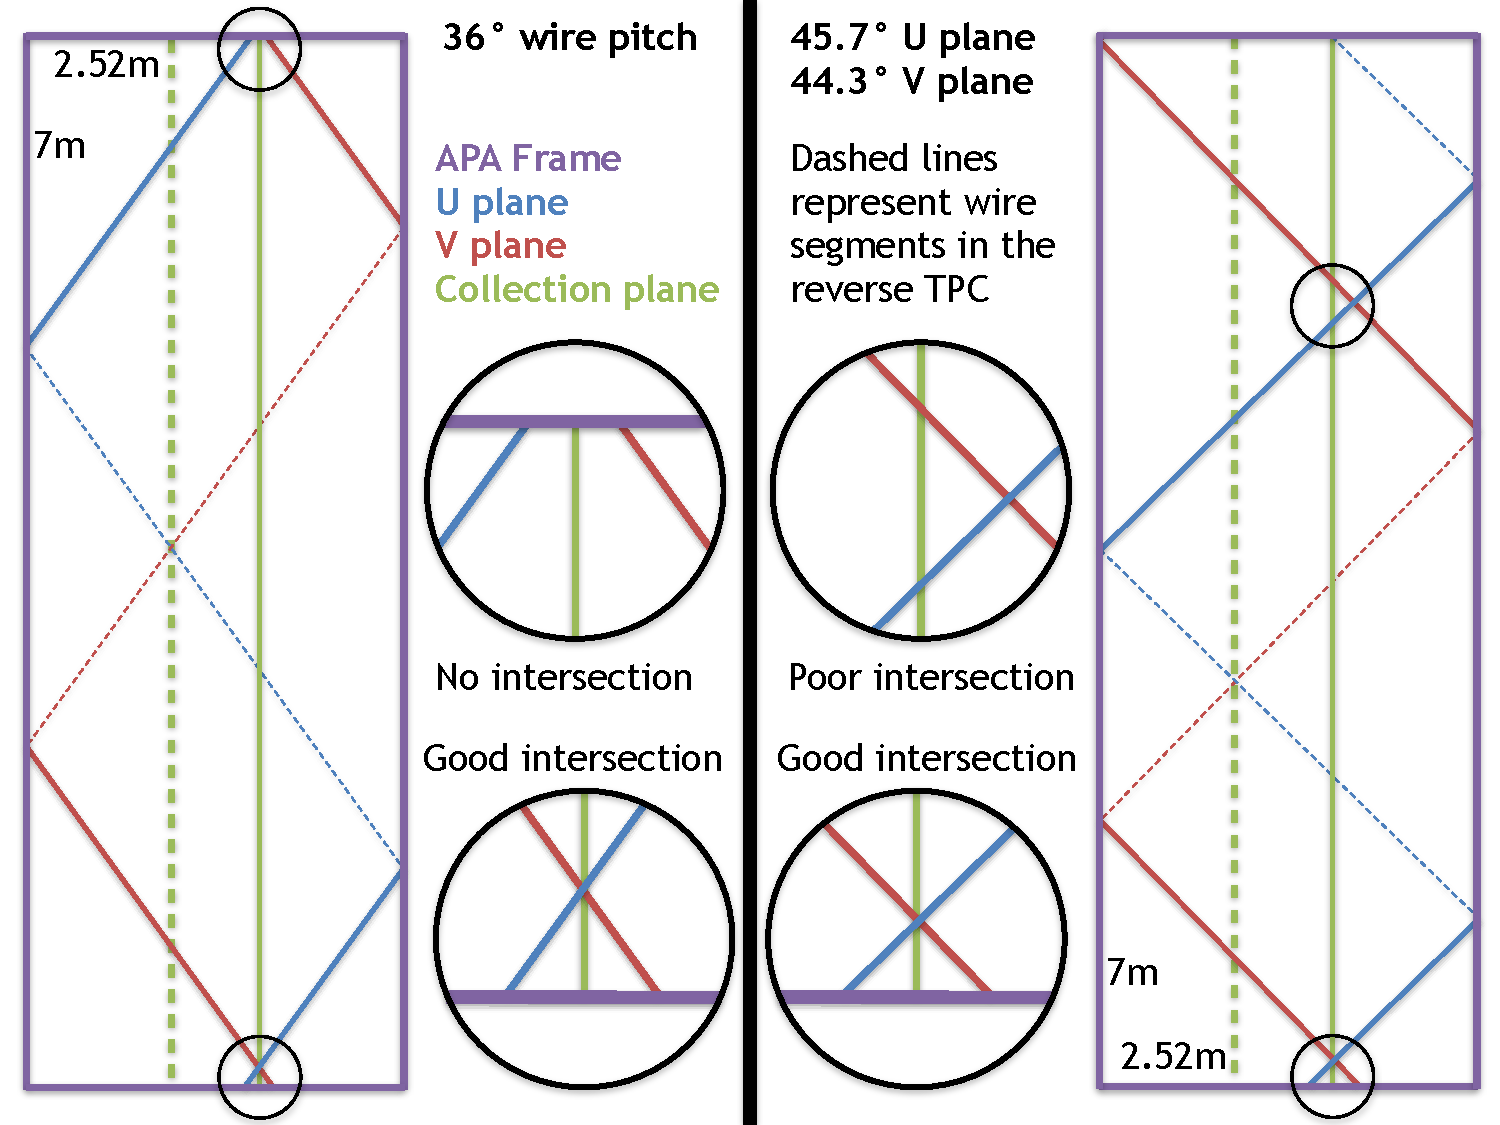
\includegraphics[width=0.85\textwidth]{WireAngleCondition}
  \caption[Performing disambiguation with different wire pitches.]
          {The effect that different wire pitches have on the ability to perform disambiguation in APAs with the far detector geometry. The left panel shows a wire pitch of 36$^{\circ}$, which is the reference design for the far detector, whilst the right panel shows wire pitches of 45$^{\circ}$ $\pm$ 0.7$^{\circ}$, as was used in the 35 ton. The left panel shows that only one 'triple point' can be made with the three wires shown, and so disambiguation is relatively trivial. The right panel shows that two 'triple points' can be made with the three wires shown, the 'triple point' where the three wires have a common intersection point is labelled as a 'good intersection' and it is this intersection point which would be chosen for the disambiguated hit.}
  \label{fig:WirePitches}
\end{figure}

Once the hits have been disambiguated they are combined to make clusters in each of the three planes, before the clusters are merged to make reconstructed tracks or showers. The clustering process is usually performed in wire-tick space on each plane separately, where all the hits from a single track or shower should be make a single cluster on each plane. It is possible to seed the start of clusters by using imaging techniques such as a Harris transform~\citep{HarrisTrans}, or to identify straight lines by using Hough transforms~\citep{HoughTrans}. As hits from a physical entity are unlikely to remain on a single channel or all come at identical times, clusters are often spread out over many channels for a range of times especially when performing clustering for showers. \\

Once clusters have been identified in each plane they can then be merged into 3-dimensional tracks and showers. The two most common tracking algorithms are PMTrack~\citep{PMTrack} and Pandora~\citep{Pandora}, and the most common showering algorithm is EMShower~\citep{EMShower}. Once 3D objects have been reconstructed, the calorimetric quantities need to be determined, this is often done separately for each plane. Two models exist for calculating $\frac{dE}{dx}$ in LArSoft, Birks model~\citep{BirksModel} and a modified Box model~\citep{PIDA_Paper} which uses a correction to the Box model~\citep{BoxModel} at low values of $\frac{dE}{dx}$. Normally the modified Box model is used as it holds for both large and small ionisation's, whereas Birks model experiences difficulties at large ionisation's and the traditional Box model struggles at low $\frac{dE}{dx}$. Both models incorporated in LArSoft, calculate the $\frac{dE}{dx}$ of a hit using the deposited charge ($dQ$) and the track pitch ($dx$) of the hit as well as the conversion of ADC value to number of electrons ($C_{GeV \rightarrow e^{-}}$), a correction due to electron lifetime ($C_{lifetime}$), the LAr density ($\rho$), the electric field ($E_{field}$) and the tunable electron recombination factors ($Recomb_{X}$). The series of equations used in Birks model are shown in Equation~\ref{eq:Birks}, whilst those used in the modified Box model are shown in Equation~\ref{eq:ModBox}. \\

\begin{subequations}
  \label{eq:Birks}
  \begin{align}
    \frac{dE}{dx} &= \frac{ dQdx }{ \alpha - (\beta \times dQdx) } \label{eq:Birks_1} \\
    dQdx &= \frac{ dQ \times C_{lifetime} }{ dx \times C_{ADC \rightarrow e^{-}} } \label{eq:Birks_Correc} \\
    \alpha &= Recomb_{A} \times C_{GeV \rightarrow e^{-}} \times 10^{-3} \label{eq:Birks_A}\\
    \beta  &= \frac{ Recomb_{B} }{ \rho \times E_{field} } \label{eq:Birks_B}
  \end{align}
\end{subequations}

\begin{subequations}
  \label{eq:ModBox}
  \begin{align}
    \frac{dE}{dx} &= \frac{ e^{\alpha} - Recomb_{A} }{ \beta } \label{eq:ModBox_1} \\
    \alpha &= \frac{10^3 \times \beta }{ C_{GeV \rightarrow e^{-} } } \times \frac{dQ}{dx} \label{eq:ModBox_A}\\
    dQdx &= \frac{ dQ \times C_{lifetime} }{ dx \times C_{ADC \rightarrow e^{-}} } \label{eq:ModBox_Correc} \\
    \beta &= \frac{ Recomb_{B} }{ \rho \times E_{field} } \label{eq:ModBox_B}
  \end{align}
\end{subequations}

When performing calorimetry it is also important that the interaction time is known so that the $x$ positions of hits can be corrected, as they will be reconstructed assuming an interaction time of 0 s. This assumption is made because when using beam events the beam trigger is placed at a time of $T = 0$. An unknown interaction time causes the hit and track positions to be calculated incorrectly, and will also skew the calorimetric corrections, as recombination is a drift dependant effect.
